\section{Spectral Method}
\begin{frame}{Spectral Method}
  Eq.(\ref{eq:polynomial_eigenvalue_problem}) can be reformulated as 
  \begin{equation} \label{eq:eigenvalue-problem}
	\mqty[ 0 & 1\\ \hat{M} & \hat{N} ]\mqty[ \tilde{v}\\ \omega \tilde{v}] = \omega\mqty[ \tilde{v}\\ \omega \tilde{v}]
\end{equation}
where the operators $\hat{M}$ and $\hat{N}$ are defined as
\begin{align*}
	\hat{M} = &-\left[(1-v_0^2)\pdv[2]{}{z} 
	-\left(3v_0 + \frac{1}{v_0}\right)\pdv{v_0}{z}\pdv{}{z}\right. \\ 
  &- \left.  \left(1-\frac{1}{v_0^2}\right)\left(\pdv{v_0}{z}\right)^2 
	- \left(v_0+\frac{1}{v_0}\right)\pdv[2]{v_0}{z}\right] \\
	\hat{N} = &-2i\left(v_0\pdv{}{z} +\pdv{v_0}{z} \right) 
\end{align*}
  Then by discretizing operators $\hat{M},\hat{N}$, this becomes an algebraic eigenvalue problem.
\end{frame}

\begin{frame}{Spectral Pollution}
  \begin{itemize}
    \item Analytical result shows all modes of Eq.(\ref{eq:polynomial_eigenvalue_problem}) with $v_0=\text{const}$ are stable.
    \item Finite-difference, finite-element, and spectral element discretization all show spurious unstable modes.
  \end{itemize}
  \begin{figure}[htbp]	
    \centering
    \begin{subfigure}[b]{0.4\linewidth}
      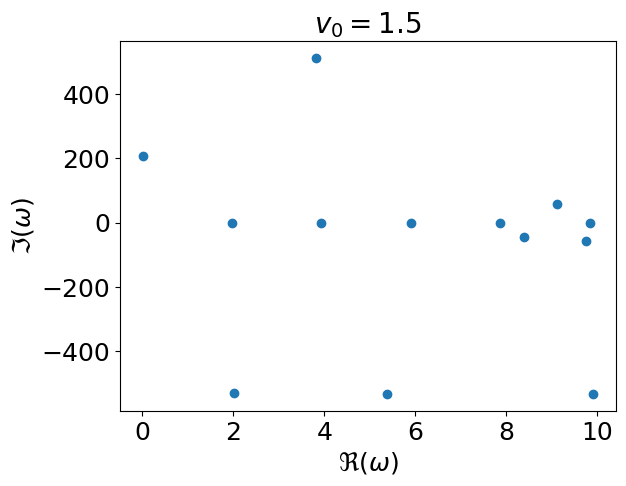
\includegraphics[width=\linewidth]{figures/eigvals-bad} 
      \caption{Unfiltered eigenvalues.}
    \end{subfigure}%
    \begin{subfigure}[b]{0.6\linewidth}
      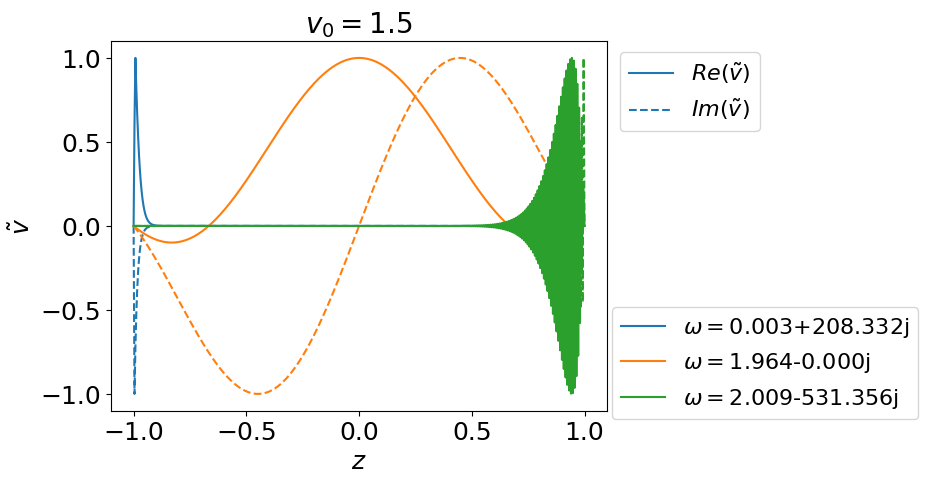
\includegraphics[width=\linewidth]{figures/eigvecs-bad} 
      \caption{First few unfiltered eigenfunctions.}
    \end{subfigure}
    \caption{Finite difference discretization was used. Spurious modes occurs regardless of the resolution.}
    \label{fig:results-bad}
  \end{figure}
\end{frame} 

\begin{frame}{Convergence Test}
  \begin{figure}
    \begin{center}
      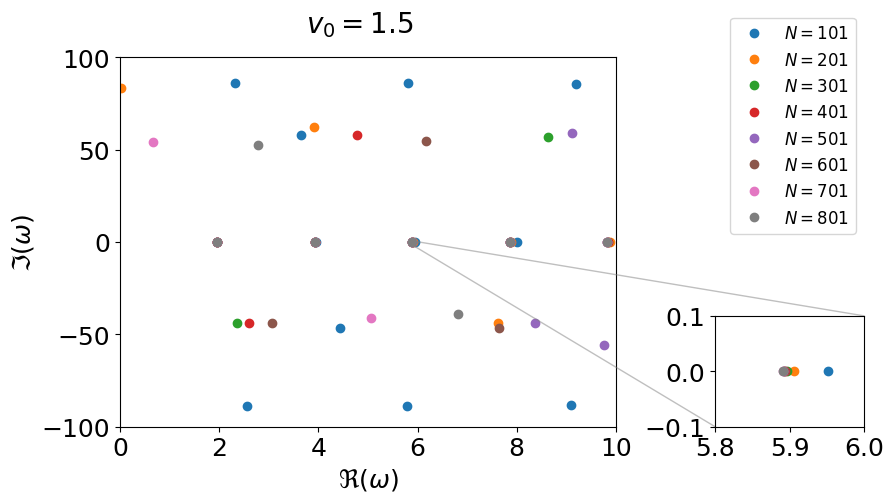
\includegraphics[width=0.9\textwidth]{figures/convergence-test.png}
    \end{center}
    \caption{Pickup the convergent eigenvalues using convergence test.}
  \end{figure}
  
\end{frame}

\begin{frame}{Filtering Spurious Modes}
  \begin{figure}[htbp]
    \centering
    \begin{subfigure}[b]{0.4\linewidth}
      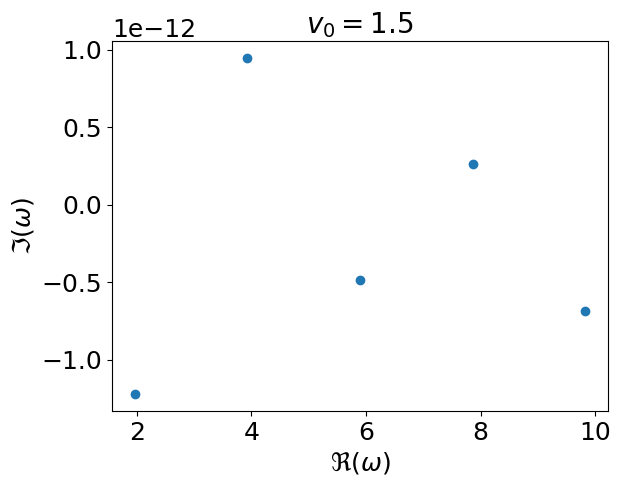
\includegraphics[width=\linewidth]{figures/eigvals-good} 
      \caption{Filtered eigenvalues.}
    \end{subfigure}%
    \begin{subfigure}[b]{0.6\linewidth}
      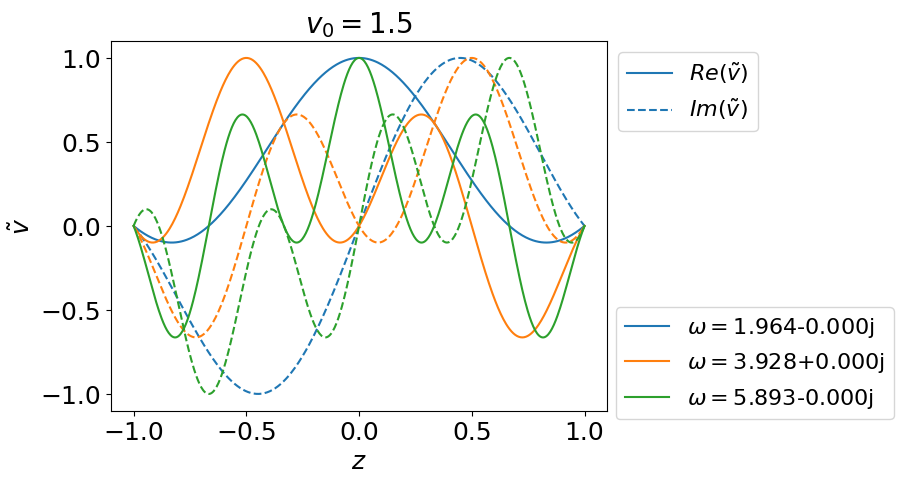
\includegraphics[width=\linewidth]{figures/eigvecs-good} 
      \caption{First few filtered eigenfunctions.}
    \end{subfigure}
    \caption{The spurious modes are changing under different resolution. We can filter them by convergence test.}
    \label{fig:results-good}
  \end{figure}
\end{frame}
